\chapter{Conceitos Básicos}
Nesta seção, serão explorados alguns fundamentos básicos para compreender, passo a passo, como será conduzida a metodologia proposta. Primeiramente, introduz-se o problema da classificação de dados. Logo após esse conceito, descreve-se como exemplos de técnicas de categorização de dados, as Redes Neurais Artificiais (RNA) e o K-vizinhos mais próximos. Por fim, é apresentado uma introdução ao Processamento de Linguagem Natural (PLN), dando enfase a um sub-conceito muito valioso para os objetivos deste trabalho, que é a classificação de texto.

\section{Classificação de dados}
Classificação de dados é um problema que abrange inúmeras aplicações em diversos tipos de cenários no nosso dia a dia, tais como diagnóstico de doenças, identificação de objetos em fotos e vídeos, categorização de seres vivos e espécies, dentre outros. Esse problema é um dos tópicos mais ativos na área de aprendizado de máquina. Classificar dados consiste em determinar um rótulo ou classe para um objeto, baseado em um conjunto de características extraídas do mesmo \citep{duda1973pattern,bishop2006pattern}. 

Em geral, cada dado é classificado como pertencente a uma única classe ou categoria. Essa forma de classificação é denominada classificação de rótulo único. Por outro lado, se houver mais uma forma de rotular a mesma entrada, então dá-se o nome de classificação de multi-rótulo. 

Formalmente, o processo de classificação consiste em: um conjunto de $i$ entradas $X = \{X_1,...,X_i\}$, um conjunto de $n$ classes $C = \{c_1,...,c_n\}$, tal que $n \geq 2$, e um conjunto de treinamento $Y = \{(X_1, \{c_1,...,c_j\}),...,(X_i, \{c_n,...,c_k\})\}$, no qual cada entrada $X_i$ é categorizada por uma ou mais classes $c_i$. O objetivo geral de um classificador é aprender, através de seu conjunto de treinamento $Y$, uma possível correlação entre os atributos das entradas com suas classes, de tal forma que para uma entrada $X' = \{X'_1,...,X'_i\}$ que não possua rótulo $c$ qualquer, seja possível classificá-la.

Para ilustrar o processo de classificação de dados, considere o problema da flor de Iris. Nesse problema, existe um conjunto de flores do gênero Iris que podem ser rotuladas de uma das três maneiras: do tipo setosa, virgínica ou versicolor. Partindo desse ponto, o objetivo é determinar a qual grupo uma determinada flor pertence baseado nas medidas de sépalas e pétalas da mesma. A Figura \ref{fig:irisExample} ilustra o processo de classificação. Inicialmente as informações específicas sobre as sépalas e pétalas devem ser extraídas em um pré-processamento. Em seguida tais medidas são processadas e suas características extraídas. Por fim, é realizada a classificação das flores. Neste exemplo os valores de $X$ serão as medidas de comprimento, largura das sépalas e pétalas e $C$ assumirá os rótulos setosa, virgínica e versicolor.

Em geral, existem diversos algoritmos para classificação de dados, em que cada um possui sua especificidade, vantagens e desvantagens. Neste trabalho, aborda-se o uso de duas técnicas clássicas para classificação de dados: Redes Neurais Artificiais (RNA) e K-vizinhos mais próximos (KNN).

\begin{figure}[ht!]
\caption{Processo de classificação de flores do gênero Iris}
\label{fig:irisExample}
\centering
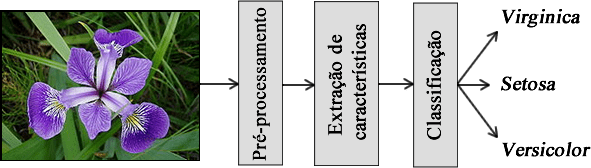
\includegraphics[scale=0.65]{img/irisExample.png}
{\fontsize{11pt}{\baselineskip}\selectfont
\\Fonte: \cite{pacheco2016agregaccao}
}
\end{figure}

\subsection{Redes neurais artificiais (RNA)}
O ser humano possui capacidades cognitivas extraordinárias e, desde o surgimento da computação, desejou-se projetar máquinas capazes de realizar tarefas inteligentes que, até então, somente eram  executadas por humanos. Os primeiros trabalhos desenvolvidos nessa área foram: um neurônio apresentado por \cite{mcculloch1943logical}, usado posteriormente como base para a concepção do  \textit{Perceptron} por \cite{rosenblatt1958perceptron} e um neurônio chamado \textit{Adaline} por \cite{widrow1960adaptive}. Tais trabalhos deram origem ao conceito da RNA que, em outras palavras, é uma tentativa de copiar a estrutura e o funcionamento do cérebro, composto este por bilhões de neurônios, para uma estrutura artificial, transformando assim as redes neurais biológicas em redes neurais artificiais \citep{Rauber2005}. Uma RNA é normalmente implementada através de um programa de computador (\textit{software}) ou através de componentes eletrônicos (\textit{hardware}).

Para compreender o conceito por trás de uma rede neural, é preciso introduzir um modelo simplificado de um neurônio e suas capacidades de processamento associadas. Cada neurônio é considerado como uma unidade básica de processamento que, quando estimulada por sinais de entrada, emitem sinais de saída como uma reação. Tais sinais, emitidos por um neurônio, são repassados para outros neurônios através de uma conexão sináptica. Tal processo pode ser repetido por várias camadas de neurônios até chegar ao nosso cérebro, que então processa essa informação e produz novas reações \citep{baeza1999modern}. A principal função de uma rede neural é armazenar conhecimento experimental e torná-lo disponível, o que em prática significa que este conhecimento é adquirido e armazenado em pesos sinápticos durante o processo.

Antes de definir e explora-se mais sobre as redes neurais, uma breve introdução a grafos é sugerida ao leitor (Apêndice \ref{app:grafos}). 

\begin{figure}[ht!]
\caption{Diagrama de um neurônio artificial}
\label{fig:graphNeuron}
\centering
\includegraphics[scale=0.5]{img/graphNeuron.png}
{\fontsize{11pt}{\baselineskip}\selectfont
\\Fonte: \cite{Rauber2005}
}
\end{figure}

Uma rede neural pode ser representada matematicamente através de uma estrutura de grafo, em que os vértices fazem o papel dos neurônios e as arestas representam as conexões sinápticas entre os neurônios. Se adicionado pesos a tais arestas, é possível mensurar a força de tal conexão sináptica. Seja $x_i$ entradas fornecidas por outros neurônios para um neurônio artificial. O processamento desse neurônio consiste em uma combinação linear das $D$ entradas, tais que $\sum_{i=1}^{D} = w_i x_i$, onde $x_i$ é uma aresta com peso $w_i$. A computação desse valor, resulta em \textit{net} (como ilustrado na Figura \ref{fig:graphNeuron}). Se o valor de \textit{net} ultrapassar um limiar $\mu$ pré-definido, uma função de ativação será executada. Neste exemplo, a função de ativação escolhida foi a Heaviside ou degrau unitário, como é comumente chamada na matemática. Por ser uma função binária, dispara $y = 1$ ou $y = 0$ na saída, de acordo com $\mu$. Além dessa função binária, existem outras alternativas, nos quais devem ser avaliadas de acordo com suas características, tais como o uso da função linear, função tangente hiperbólica, função arco tangente, função sigmóide, dentre outras.
 
Geralmente o uso de somente um único neurônio não é suficiente para a efetuação de tarefas de classificação mais complexas, necessitando assim, do uso conjunto de outros neurônios, nos quais operem em paralelo a este, aumentando assim a capacidade de processamento da rede neural. A partir disso, surge o conceito de organização dos neurônios em camadas \citep{duda1973pattern, bishop2006pattern, martin2018speech}. Camadas estas que, quando não ligadas diretamente às entradas e nem às saídas da rede, chamam-se camadas escondidas ou ocultas (do inglês: \textit{Hidden layers}). 
 
Uma categorização fundamental da topologia dos neurônios pode ser feita em relação ao método escolhido para a propagação da informação recebida, ou em outras palavras, quem receberá a informação processada pelo último neurônio. Pode-se distinguir então, de duas formas, entre redes de propagação para frente (do inglês: \textit{Feed-Forward Network} - FFN) e redes realimentadas (do inglês: \textit{Recurrent Neural Networks} - RNN), ver Figura \ref{fig:graphNeuron2}.
 
 \begin{figure}[ht!]
\caption{Diagramas que representam redes \textit{Feed-Forward Network} e \textit{Recurrent Neural Networks}}
\label{fig:graphNeuron2}
\centering
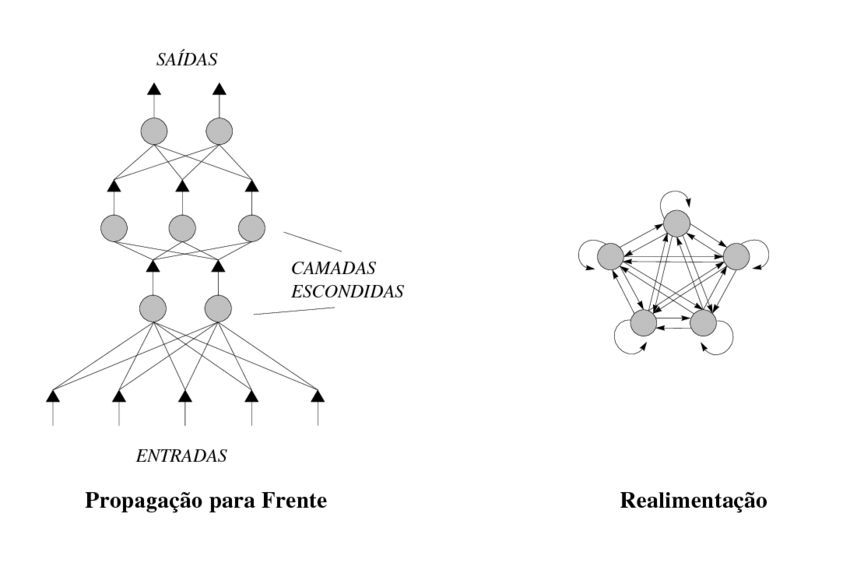
\includegraphics[scale=0.5]{img/graphNeuron2.png}
{\fontsize{11pt}{\baselineskip}\selectfont
\\Fonte: \cite{Rauber2005}
}
\end{figure}
 
Uma \textit{Feed-Forward Network} é uma rede multicamadas unidirecional, no qual não existe um ciclo entre as camadas de neurônios, ou seja, após o processamento de uma camada, as informações são sempre repassadas adiantes, para as sucessoras camadas, até a camada de saída, nunca sendo possível o retorno para camadas já executadas. Redes de propagação para frente, também chamadas de \textit{Multilayer Perceptron - MLP}, é a topologia de neurônios mais utilizada e estudada na área de aprendizado de máquina. As redes FFN são comumente aplicadas para o reconhecimento de padrões e classificação de dados.
 
Uma \textit{Recurrent Neural Networks} é uma rede que possui arestas entre os seus neurônios sem restrições, em que o comportamento dinâmico desempenha um papel fundamental nesse modelo. Em alguns casos, os valores de ativação da rede passam por um processo de relaxação, por múltiplos e até repetidos neurônios, até chegarem a um estado estável. Difere, principalmente, das redes FNN por possuir uma conexão com suas decisões passadas, em que cada saída pode ser tratada com uma nova entrada, armazenando conhecimento. É uma topologia poderosa e ao mesmo tempo complexa, tradicionalmente difícil de ser treinada. As redes RNN vêm sido aplicadas com grande sucesso para o processamento de linguagem natural, com ênfase em textos e falas.

Uma propriedade relevante das redes neurais é sua habilidade de aprender a partir do ambiente a qual foi inserida, também chamado de ambiente de aprendizado, em que sua capacidade de aprender é sucessivamente melhorada através do processo de adaptação dos parâmetros livres (pesos sinápticos e limiares) de sua rede. Este aprendizado pode ser adquirido de várias formas \citep{bishop2006pattern, duda1973pattern, Rauber2005}. Duas formas de aprendizado comuns são: aprendizagem supervisionada, em que o conhecimento é transmitido por meio de exemplos de entrada e saída; e aprendizagem não-supervisionada, no qual a rede só dispõem dos valores de entrada e deve descobrir as correlações entres os exemplos de treino.

Um método amplamente utilizado para o treinamento e aquisição de aprendizagem para redes FNN é o algoritmo de retro-propagação do erro (do inglês: \textit{Backpropagation}) proposto por \cite{werbos1974beyond}, baseado na regra de aprendizagem por correção de erro. Neste algoritmo (ilustrado na Figura \ref{fig:backpropagationExample}), a aprendizagem se consiste em dois passos através das diferentes camadas da rede: um passo para frente (propagação), no qual os pesos sinápticos da rede estão fixos, repassando os sinais funcionais normalmente desde a entrada até a saída; e um passo para trás (retro-propagação), em que cada saída gerada por um neurônio é subtraída da resposta real da rede, produzindo assim um sinal de erro, propagado em direção inversa as arestas da rede. O objetivo desse algoritmo é ajustar os pesos sinápticos da rede de forma que, a resposta real obtida, se aproxime ao máximo da desejada, ou seja, minimizar o erro gerado pela processamento da rede.

\begin{figure}[ht!]
\caption{Algoritmo \textit{Backpropagation} para treinamento de redes \textit{Feed-Forward Network}}
\label{fig:backpropagationExample}
\centering
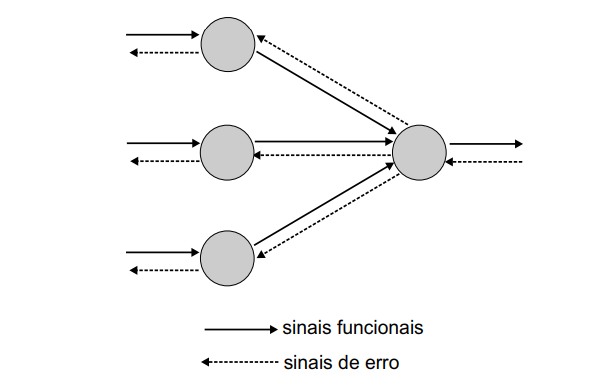
\includegraphics[scale=0.75]{img/backpropagationExample.png}
\end{figure}

Já para treinar uma rede RNN, o algoritmo de treinamento é baseado no \textit{Backpropagation}, chamado de \textit{Backpropagation Through Time - BPTT}. Que assim como o seu primitivo, calcula o erro gerado por cada neurônio, adaptando os pesos sinápticos. Como diferencial, a variável tempo é adicionada a cada passo. O que em prática significa, que para cada vez que é executado a retro-propagação do erro, uma camada cópia é gerada e deverá ser levada em consideração no próximo passo. Este algoritmo tende a ser computacionalmente custoso para cada novo passo dado, devido ao fato da ordem do erro aumentar a cada execução. Podendo reduzir os valores dos pesos a zero, como também crescerem exponencialmente, resultando em uma aprendizado lerdo e sujeito a ruído. Uma solução alternativa para este problema é o algoritmo aproximado \textit{Truncated BPTT}, no qual um limite de passos a serem considerados é definido, reduzindo assim o custo total de computação para sequências longas.
 
Por ser uma ferramenta poderosa, flexível e possuir uma grande capacidade de processamento, vem apresentando resultados excepcionais nas mais diversas aplicações da literatura \citep{gupta2018text, martin2018speech, bishop2006pattern, duda1973pattern, Rauber2005}, justificando assim a sua escolha como classificador de dados para este trabalho. 

Por outro lado, devido a sua complexidade e alto custo computacional, pode ser um obstáculo a ser enfrentado. Supondo que existam $n$ exemplos de teste, com $m$ características, $k$ \textit{Hidden layers}, no qual cada uma contém $h$ neurônios e existam $p$ neurônios de saída. O tempo total de execução do algoritmo de \textit{Backpropagation} para uma MLP seria $\mathcal{O}(n*m*h^{k}*p*i)$, no qual $i$ é o número de iterações executadas.

\subsection{K-vizinhos mais próximos}
O algoritmo K-vizinhos mais próximos (do inglês: \textit{K-neareast neighbours} - KNN) tem como objetivo determinar o rótulo de classificação de uma amostra, baseando-se em outras amostras vizinhas, advindas de um conjunto de treinamento. O classificador KNN, um dois mais simples e, ao mesmo tempo, um dos mais eficazes, dentre os algoritmos de classificação, é baseado em instâncias. Esse algoritmo encontra os $k$ objetos mais similares ao termo de consulta e realiza uma votação de acordo com as classes às quais pertencem esses $k$ objetos, assinalando por fim, uma classe ao objeto de teste. A literatura apresenta diversas formas para expressar essa distância/similaridade dentre os objetos de análise \citep{fukunaga1975knn, duda1973pattern}. Por exemplo, se os dados trabalhados estão em formato de texto, é comum utilizar a similaridade por cossenos. Por outro lado, se os dados possuírem formato numérico, possivelmente a distância euclidiana será mais eficaz.

\begin{figure}[ht!]
\caption{Ilustração do algoritmo K-vizinhos mais próximos aplicado em um plano cartesiano}
\label{fig:knnExample}
\centering
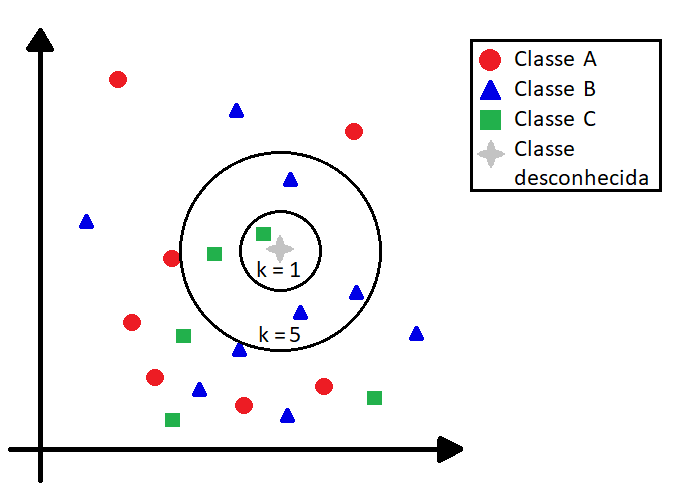
\includegraphics[scale=0.5]{img/knnExample.png}
{\fontsize{11pt}{\baselineskip}\selectfont
\\Fonte: Elaborado pelo autor
}
\end{figure}

Na Figura \ref{fig:knnExample}, é ilustrado o processo de classificação com o algoritmo KNN. Neste exemplo, têm-se três classes, anteriormente conhecidas, sendo elas: classe A (círculo vermelho), classe B (triangulo azul) e classe C (quadrado verde). O objetivo é identificar, por similaridade, a qual classe pertence a amostra (estrela cinza), olhando para o seus $k$ vizinhos mais próximos. Para $k = 1$, esse algoritmo classificaria a amostra como pertencente a classe C. Por outro lado, se o valor escolhido para $k$ é $5$, por votação majoritária, a amostra seria classificada como pertencente a classe B.

Um grande fator que pode definir a eficácia do algoritmo KNN no contexto em que é aplicado, é o valor de escolha para o $k$. Por ser um valor variável (não constante), deve ser determinado de forma empírica, variando de acordo com a base de dados. Caso o valor escolhido para $k$ seja muito baixo, a classificação ficará sujeita a \textit{outliers}, ou seja, dados atípicos ou ruídos, que não condizem com o contexto da classificação. Já por outro lado, se $k$ assumir um valor alto, a vizinhança poderá incluir elementos pertencentes a outras classes, não necessariamente relevantes ao objeto de análise, interferindo assim, no resultado final da rotulação \citep{fukunaga1975knn}. Por ser um fator relevante, deverá ser avaliado cuidadosamente.

\section{Processamento de linguagem natural}
O processamento de linguagem natural (PLN) têm como objetivo tratar os mais diversos aspectos presentes dentro da comunicação humana, tais como sons, palavras, sentenças e discursos, levando em consideração os seus formatos, referências, estruturas, significados, contextos e aplicações. Embora exista outros animais que possuem um vocabulário com centenas de sinais, tais como os elefantes e os golfinhos, somente os seres humanos possuem a capacidade de se comunicar, de forma confiável, em um número ilimitado de mensagens qualitativamente diferentes, sobre um tema qualquer \citep{russell1994inteligencia, gonzalez2003recuperaccao}.

Hoje em dia, com o constante crescimento da rede mundial de computadores, possibilitou o acesso a enumeras páginas de informações na \textit{Web}, no qual quase todas elas estão em um formato de linguagem natural. Entretanto, disponibilidade não significa fácil acesso à informação. Para uma máquina adquirir tal conhecimento, ela precisa ser treinada, de forma exaustiva, para compreender as complexas, e muitas vezes ambíguas, linguagens em que os seres humanos se comunicam.

Segundo \cite{russell1994inteligencia}, as linguagens naturais, tais como o português e o espanhol, não podem ser caracterizadas como um conjunto de sentenças definitivas, pois de acordo com o contexto em que for definida uma sentença de alguma dessas linguagens, ela pode possuir inúmeras interpretações diferentes. Portanto, convém definir um modelo de linguagem natural como uma distribuição de probabilidade sobre sentenças. Existe um famoso ditado popular brasileiro que diz "para um bom entendedor, meia palavra basta", o que pode ser comumente aplicado para nós humanos, que possuímos uma espécie de dispositivo de especialização para aquisição de linguagens \citep{chomsky2014aspects}. Já que meia palavra basta, pode-se concluir que uma sentença de uma linguagem natural não é sempre aleatória, e que sim possui algum grau de previsibilidade e correlação entre a escolha das palavras. Portanto, nos leva a acreditar que palavras similares estejam presentes no mesmo contexto.

O PLN consiste no emprego de um conjunto de técnicas computacionais para aprender, entender e reproduzir uma linguagem natural. No processo de tradução do significado, tratamento de ambiguidade e entre outros desafios, o PLN pode utilizar de conhecimentos linguísticos e métodos estatísticos para resolvê-los. Por exemplo, considere uma análise sobre dois textos semelhantes A e B, no qual desconfia-se que exista possibilidade de plágio. Com o uso de um pré-processamento, seria possível filtrar os textos para remover \textit{Stopwords}, que são palavras funcionais, tais como artigos, preposições e conetivos, que quando analisadas individualmente não possuem grande relevância para o contexto. Após o pré-processamento, é possível aplicar um método da distância mínima de edição, que como o próprio nome diz, significa quantas operações de inserções, remoções ou substituições de caracteres são necessárias para que o texto A torne-se o texto B, ou vice-versa. 

Uma das tarefas possíveis no PLN é a classificação de texto. Para compreender melhor o processo de aplicação de conhecimentos linguísticos para essa tarefa, é apresentado a seguir uma seção sobre classificação de texto.

\subsection{Classificação de texto}
Segundo \cite{aggarwal2014data} um dos principais desafios encontrados durante o processo de classificação de texto é sobre o tamanho dos dados tratados, que podem variar de algumas poucas dezenas para milhões de palavras. Esses dados se encontram, quase sempre, de maneira esparsa, ou seja, possuindo baixa frequência de uso. Por outro lado, têm-se muitas vezes uma alta frequência de dados não úteis para tratamento, como as \textit{Stopwords}.

É comum também, dependendo do contexto ou de como obteve-se o texto, que exista palavras com o mesmo significado, erros ortográficos ou até mesmo erros de codificação. Logo, muitas vezes é necessário uma etapa de normalização do texto. Normalizar um texto significa, segundo \citep{martin2018speech}, converte-lo dê forma conveniente à um formato padrão, que facilite as manipulações sobre os dados. Exemplos de sub-etapas da normalização são: \textit{tokenization} e \textit{lemmatization}. 

Na \textit{tokenization}, deseja-se separar as palavras contidas em um texto, de maneira que elas fiquem isoladas. Por exemplo, na frase "fui ao Rio de Janeiro", resultaria em 5 \textit{tokens} distintos: "fui", "ao", "Rio", "de", "Janeiro". Contudo, uma separação em \textit{tokens} por somente o uso do espaçamento em branco, nem sempre representa o contexto da frase, pois como no exemplo "fui ao Rio de Janeiro", Rio de Janeiro não deve ser tratado como três \textit{tokens} distintos, e sim como um único \textit{token}, que no caso representa a cidade ou estado brasileiro. Em algumas linguagens naturais, nem todas palavras possuem espaço entre si, como é o caso do mandarin da China, por exemplo, dificultando ainda mais o processo de \textit{tokenization}. 

A etapa de \textit{lemmatization}, é o processo, efetivamente, de deflexionar uma palavra para determinar o seu lema. Por exemplo, as palavras gato, gata, gatos, gatas são todas formas do mesmo lema: gato. Igualmente, as palavras estudou, estudava, estudaria, estudará, são do mesmo lema: estudar. A lematização é útil quando deseja-se ver os usos de palavras em contextos sem importância das flexões, como também para a criação e uso de índices ou na investigação linguística. Por poder se tornar um processo custoso, dependendo da quantidade de dados, uma alternativa mais barata acaba sendo mais viável nesses cenários. Surgindo então o conceito de uma análise morfológica, chamada \textit{stemming}.

No \textit{stemming}, deseja-se reduzir as palavras flexionadas, ou às vezes derivadas, ao seu tronco, base ou raiz, cortando assim caracteres dos seus sufixos. Por exemplo, a stemização das palavras estudou, estudava, estudaria, estudará, será "estud", visto que é o prefixo comum e redutível por todos. Um dos algoritmos mais conhecidos para \textit{stemming} é o Porter, proposto por \citep{porter1980algorithm}. Se por um lado, facilita a identificação de variantes para um mesmo lema e possui o potencial de lidar com palavras desconhecidas, transformando-as em uma semelhante conhecida, pelo outro lado, a utilização deste método pode gerar erros de interpretação, tanto quando ele corta demais as palavras, como também quando ele não corta o suficiente, permanecendo a ambiguidade.

Além de uma etapa de normalização dos dados, uma etapa para extração e seleção de características é essencial, e pode gerar benefícios como: redução da dimensão do problema, que por sua vez aumenta a velocidade de execução do algoritmo; redução na quantidade total de características; aumento na precisão de predição e acerto; e facilitar a visualização dos dados.

Uma vez escolhido um conjunto de características, é possível aplicar algumas técnicas de classificação de texto, inclusive duas das que já foram abordadas aqui, as redes neurais artificiais e o k-vizinhos mais próximos, nos quais apresentam uma precisão superior a 98\% quando aplicados ao problema de identificação de \textit{e-mail spam} \citep{russell1994inteligencia}.

A classificação ou categorização de texto é portanto a tarefa de, dado algum tipo de texto, decidir a qual conjunto predefinido de classes o mesmo pertence. Por exemplo, decidir a qual linguagem pertence uma sentença ou identificar se um texto de uma chamada de emergência é falsa ou não, são exemplos de classificação de texto.